%======================================================================
\chapter{Model Development}
%======================================================================
\section{Introduction}
In this thesis, the objective is to develop a numerical model to simulate the residual stress and  dislocation density found in Si wafers produced for solar cell applications. The manufacturing process involves casting via directional solidification and then wire sawing. Both process steps involve significant thermal loads and mechanical deformation. In order to determine the material state after wire sawing, it is important to solve the temperature-time and the stress-strain mathematical equations simultaneously. Solving these equations is challenging because they require accurate material properties, boundary conditions, geometry and state equations (for stress and dislocation). These material properties can vary significantly depending upon the purity and grain structure of silicon. The boundary conditions and geometry can vary depending on the physical setup for which the process is being simulated. 

Mathematical equations for any physical process such as temperature evolution and mechanical deformation can be solved using numerical methods. One of the most commonly used numerical methods for solving problems related to continuum mechanics is finite element analysis (FEA). In this research project, the commercial finite element software package ABAQUS 6.12 has been used to model the processing of Si wafers. This software is an efficient explicit/implicit finite element simulation package with excellent capability to solve transient heat transfer problems and mechanical deformation problems, and is very well documented. 

\section{Model Formulation, Domain \& Geometry}


\subsection{Analysis Formulation}

The finite element prediction of the residual stress and dislocation density after directional solidification and wire sawing requires solving the heat transfer and stress-strain partial differential equations. The heat transfer equation during solidification is simplified by neglecting solute convection;  heat conduction is assumed to be the only heat transport medium. The heat transfer equation in the standard form used in the finite element formulation is given by,
\begin{equation}
   \frac{\partial(\rho c_{p} T)}{\partial t} 
   - \nabla\cdot(k\nabla T)
   = \dot{Q}
   \label {heat_eq}
\end{equation}
\newline
where $\rho$ is the density in \SI{}{kg.m^{-3}}, $c_{p}$ is the specific heat in \SI{}{J.kg^{-1}.K^{-1}}, $T$ is the temperature, $k$ is the thermal conductivity in \SI{}{W.m^{-1}.K^{-1}}, and $\dot{Q}$ is the heat generated inside the domain in \SI{}{W. m^{-3}}. In case of solidification model, the term $\dot{Q}$ represents the latent heat. This equation is discretized and then solved to obtain the temperature-time distribution across the domain. 

The main stresses during casting and wire-sawing arise from thermal strains that occur as a result of temperature variations across the domain (if the pressure from the wire is ignored). These thermal strains are then used to calculate the residual stress and dislocation density. The governing equation defining this problem is the equation of motion given by,
\begin{equation}
  \nabla^{}\cdot\sigma_{S} + b
   = 0
   \label {continuity_eq}
\end{equation}
where $\sigma_{S}$ and $b$ represent the stress and the acting body force at any point inside the domain respectively. 

If the strains are small, and deformation is within the elastic regime, then the stress tensor $(\sigma)$ and the strain tensor $(\epsilon)$ have a linear dependence proportional to a stiffness matrix $[D^{el}]$ as per Hooke's law, 
\begin{equation}
  (\sigma)
   = [D^{el}] (\epsilon^{el})
   \label {Hookes_law}
\end{equation}
where the matrix [$D^{el}$] contains the material elastic constants that are a function of elastic modulus and Poisson’s ratio. Beyond the elastic regime, the relation between stress and strain is no longer linear and thus [$D$] depends upon the respective constitutive behavior of the material. In finite element analysis, this is simulated incrementally, i.e.,
\begin{equation}
  d\sigma
   = D^{ep} d\epsilon^{ep}
   \label {Hookes_law_partial}
\end{equation}
where $d\sigma$ and $d\epsilon$ represent the increment of stress and strain, and [$D^{ep}$] represents the inelastic constitutive behaviour of the material.

The ABAQUS software contains four built-in constitutive models: elastic-plastic, elastic-viscoelastic, elastic-creep and elastic-creep-plastic. As discussed in the literature review, the constitutive behaviour of Si during casting and wire-sawing is majorly governed by islocation creep deformation, and so the elastic-creep ABAQUS scheme is used in this thesis. A custom  subroutine has been written in FORTRAN 77 to implement the disllocation creep model. This will be discussed later in the document. 

Within ABAQUS, thermal-mechanical FEA can be performed in one of two ways. First, known as fully-coupled analysis, the heat transfer and stress-strain equations are solved simultaneously. Second, known as sequential coupling analysis, the heat transfer equation is solved first and its results are then applied to the mechanical model when solving the stress-strain equations. The first option is used when the heat transfer and the stress-strain equations have a strong mutual dependence. The second option is used when the interaction can be approximated as one way i.e. the stress-stress equation is dependent on the heat transfer equation.

In finite element methods, the correctness of a solution is determined by how small are the residual values. These residual values are mathematical functions of expected and calculated solution values. In any type of analysis, at each increment, the ABAQUS solver does several iterations till residual $R$ is close to 0 within an error tolerance  $\epsilon$. This is called a convergence criteria,
\begin{equation}
||R||<\epsilon
\label {residualsl}
\end{equation}

Mathematically, the fully coupled analysis can be written as, 
\begin{equation}
\begin{bmatrix}
K_{uu} &  K_{uT} & \\ 
K_{Tu} &  K_{TT} & \\ 
\end{bmatrix} 
\begin{pmatrix}
\nabla u\\ 
\nabla T
\end{pmatrix}
= 
\begin{pmatrix}
R_{u}\\ 
R_{T}
\end{pmatrix}
\label {coupled_anal}
\end{equation}
where $\nabla u$ and $\nabla T$ are the respective corrections to the incremental displacement and temperature, $K_{ij}$ are components of the unsymmetric Jacobian matrix and $R_{i}$ are mechanical and thermal components of the residual vector. ABAQUS solves this coupled system using the Newton-Raphson method with the heat transfer and the strain-strain differential equations solved using backward-difference scheme.

In case of a weak coupling or a sequentially coupled analysis, the off-diagonal submatrices $K_{uT}$ are $K_{Tu}$ are small compared to the components in the diagonals in the Jacobian matrix of Equation \ref{coupled_anal}. The off-diagonal components can be set to 0 as shown,
\begin{equation}
\begin{bmatrix}
K_{uu} &  0 & \\ 
0 &  K_{TT} & \\ 
\end{bmatrix} 
\begin{pmatrix}
\nabla u\\ 
\nabla T
\end{pmatrix}
= 
\begin{pmatrix}
R_{u}\\ 
R_{T}
\end{pmatrix}
   \label {sq_coupled_anal}
\end{equation}
Due to this approximation, the thermal and the mechanical equations can be solved separately and more efficiently, reducing computation time.

The main issue with sequential coupling in this project is the need to take extra precautions while solving the stress-strain equations since the stress fields, which are linked to the generation of dislocations, are very sensitive to temperature changes. Under such temperature-dependent kinematical framework, even a small error in the temperature field might introduce large errors in the stress-strain fields and hence a high level of accuracy in temperature is required. In this work, errors in the temperature are minimized by enforcing a small maximum time steps of 2s in the thermal model. This considerably increased the processing time but ensured accuracy. The overall scheme was implicit.

\subsection{Model Domain, Geometry and Meshing}

\subsubsection{Casting}

The analysis for directional solidification assumed that the mc-Si casting was cylindrical, and was being performed in a Crystalox DX-250 furnace, with dimensions 250mm in diameter and 105mm in height. The goal was to characterize the thermal evolution of the ingot during directional solidification, along with the residual stress and dislocation density states at the end of the casting process. Due to symmetry along the centreline, the finite element analysis is only required for a one-half radial section having dimension of 125mm by 105mm. Further, this approach converted the problem of solving the heat and mechanical equations in 3D into a axi-symmetric, saving computational time. The geometry was meshed with 1548 nodes and 1470 elements with each element having four nodes. The element types used for thermal and stress models were axisymmetric diffusive heat transfer element and axisymmetric reduced-integration solid element given by DCAX4 \& CAX4R respectively in ABAQUS. This mesh is shown in Figure \ref{fig:casting-mesh}.

This objective of this analysis was also to study the residual stress and the dislocation density under slow, medium and fast cooling. This however required the correct value of the convective heat transfer coefficient of the bottom surface via which the heat was escaping from the ingot. Under the lack of this critical information, the cooling was simulated by assuming the bottom surface to cool at 2, 5 and 8 K/Min, mimicking slow, medium and fast colling respectively. The time supplied for simulation was, therefore,  900, 300 \& 200 minutes respectively for slow, medium and fast cooling. The extra time was supplied in the cooling simulations to ensure that all the points in the domain have reached 298 K and there is no final temperature gradient inside the domain. The term residual stress is different from stress and it refers to that stress which is present inside the domain after all type of load has been removed, thermal in this case. This is why it is important that there is no final thermal gradient inside the ingot. 

This cooling scheme is a very lose approximation of the real cooling phenomenon but the way this simulation scheme is developed, a complex heat transfer coefficient can be be fed into this scheme to obtain better results in the future.


\begin{figure}[h]
    \centering
    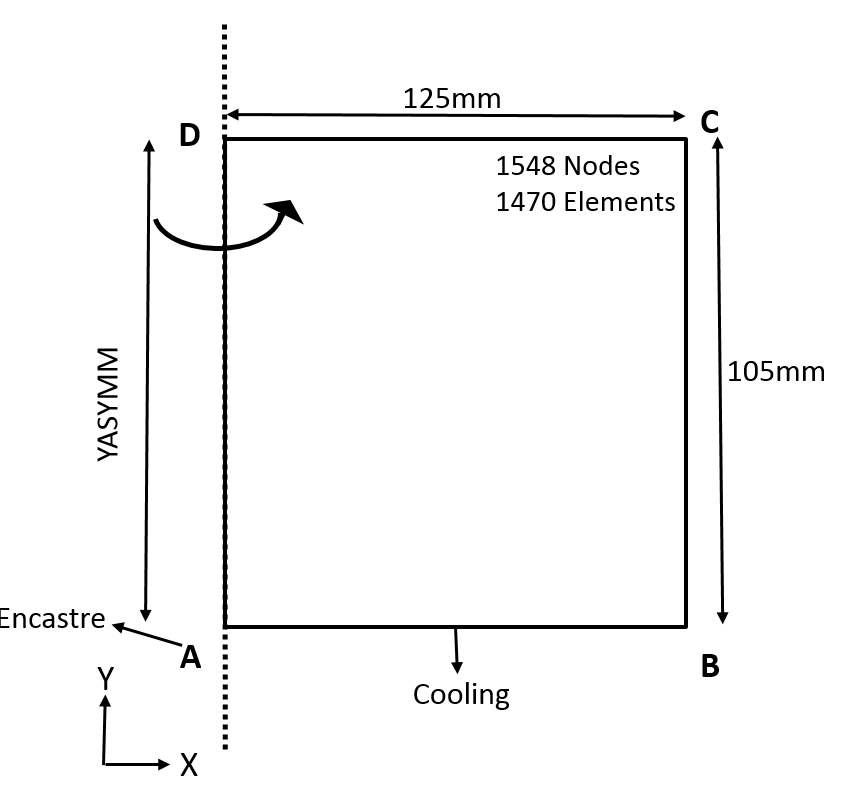
\includegraphics[width=4.0in]{casting-mesh.PNG}
    \caption{Mesh for casting simulation}
    \label{fig:casting-mesh}
\end{figure}

\subsubsection{Wire Sawing}
The analysis domain for wire sawing model was a circular volume with diameter 250 \SI{}{mm} and height 1500 \SI{}{\micro.m}. The goal was to determine the amount of warpage and dislocation density in as-cut Si wafers taken from different heights along the ingot. The wire sawing simulations were performed on three different locations within the casting: 26.25, 52.5, and 79.75 \SI{}{mm} from the base of the ingot. The reason for performing the analysis on these sections instead of the whole ingot was to minimize computational cost and time. The caveat of this approach is the need to correctly map stress, strain and dislocation density from the casting model onto these sections. The first step was to map the stress, displacement, and dislocation density fields from the results of the casting simulation as initial conditions. Once mapped, the next steps were to perform the thermal and mechanical simulations. For all the three sections, only a single thermal model was built because it was assumed that the temperature profile while multi-wire sawing does not vary along the axis of the ingot. The mechanical models were built separately for these three sections, and applied the temperature results from the thermal simulation as a pre-existing field. The time for wire sawing was taking as 500 minutes since, industrially, this is the time that it takes for multi-wire sawing of Si ingots.  

An axisymmetric mesh could not be used for modelling wire sawing because it is not a symmetric operation. A special type of mesh, as shown in Figure \ref{fig:wiresawing-mesh}, was constructed by writing a script in PYTHON. This mesh had parallel lines perpendicular to the feed movement direction. This meshing was used to simulate a material removal pattern with wire movement from the entry point to the exit point. Note that, this mesh is still an approximation to wire sawing since in reality the wire bows while slicing. This mesh had 9608 nodes and 6903 elements with 8 nodes per element for both the thermal and stress models. The 3D diffusive heat transfer DC3D8 and continuum C3D8 elements were used for the thermal and mechanical model respectively.

\begin{figure}
    \centering
    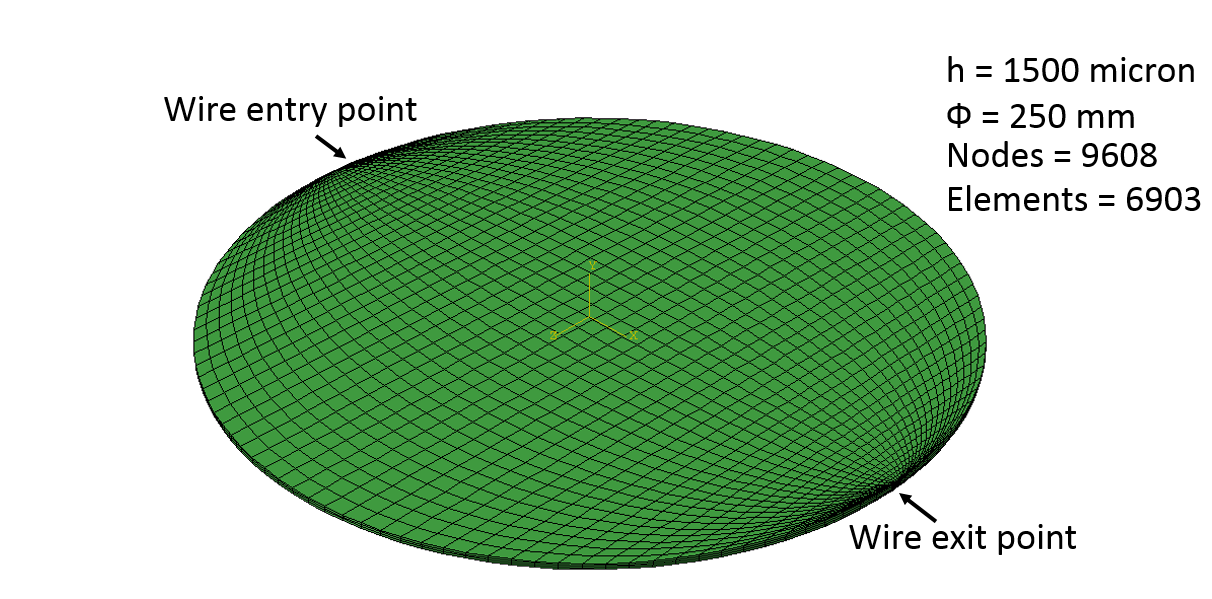
\includegraphics[width=5.0in]{wiresawing-mesh.PNG}
    \caption{figure}{Mesh for wire sawing simulation}
    \label{fig:wiresawing-mesh}
\end{figure}

\section{Input Material Properties}

\subsection{Thermal Properties}
The thermal properties of liquid and solid silicon, required for performing the temperature finite element analysis, include: density, latent heat of fusion, heat capacity, and thermal conductivity. These are tabulated along with their respective sources in \ref{table:thermal-prop-1} and \ref{table:thermal-prop-3}. Impure materials usually solidify over a range called as liquidus-solidus temperature range depending upon the concentration of primary and secondary constituents in it. For a material with high concentration of one constituent, the liquidus-solidus range is small. During directional solidification of mc-Si from MGS, due to the 98\% purity of silicon, this range is between $0.5-1\degree C$ around the melting point temperature i.e. $1410\degree$C. Thermal conductivity of silicon depends on temperature \cite{glassbrenner1964thermal} and changes significantly from room temperature to its melting point.

\begin{table}[h]
    \centering
    \begin{tabular}{|c|c|}
    \hline
    $T_{solidus}$ (\SI{}{K}) & 1682.5 \\ 
    \hline
    $T_{liquidus}$ (\SI{}{K}) & 1683 \\
    \hline
    Latent Heat (\SI{}{kJ.kg^{-1}}) & 1926 \\
    \hline
    \end{tabular}
    \caption{Thermal property of Si \cite{}}
    \label{table:thermal-prop-1}
\end{table}

\begin{table}[]
    \centering
    \begin{tabular}{ |c|c|c|c|}
    \hline
    $T$ (\SI{}{K}) & $k$ (\SI{}{W.m^{-1}.K^{-1}}) & $T$ (\SI{}{K}) & $k$ (\SI{}{W.m^{-1}.K^{-1}})  \\
    \hline
    200 & 266 & 1000 & 31 \\
    \hline
    300 & 156 & 1100 & 28 \\ 
    \hline
    400 & 105 & 1200 & 26 \\
    \hline
    500 & 80 & 1300 & 25 \\ 
    \hline
    600 & 64 & 1400 & 24 \\ 
    \hline
    700 & 52 & 1500 & 23 \\ 
    \hline
    800 & 43 & 1600 & 22 \\ 
    \hline
    900 & 36 & 1681 & 22 \\ 
    \hline
    \end{tabular}
    \caption{Specific heat of Si with Temperature \cite{}}
    \label{table:thermal-prop-3}
\end{table}

Silicon has a unique liquid-solid density change property, unlike other elements, as liquid silicon is denser than solid silicon meaning that solid Si has the potential to float during solidification. However, for this analysis, this material behavior is ignored to reduce complexity. The variation in density with temperature for solid Si is also ignored because adding that feature to the model would change the mass balance of the system.



\subsection{Mechanical Properties}
The mechanical properties required for performing the stress finite element analysis are: density, elastic moduli, Poisson’s ratio, thermal expansion, and dislocation creep behavior. These properties are tabulated in table \ref{table:mech-prop-1}, along with their respective sources.

\begin{table}[]
    \centering
    \begin{tabular}{ |c|c|c|c| } 
    \hline
    Property & Temperature range (K) & Value\\
    \hline
    $\alpha(T)$ (\SI{}{K^{-1}})  & 298$<T<$1683 & 3.725$\times 10^{-6} \cdot [1-e^b]$\\
     & & $b=-5.88 (T-124) 10^{-3}+5.55 T 10^{-4}$\\    
    & 1683 $<T$ & 0  \\
    \hline
    $\rho$ (\SI{}{kg.m^{-3}}) & N/A & 2330 \\
    \hline
    E (\SI{}{G.Pa}) & 298$<T<$ 1683 & $1.7 \times 10^{11} - 2.771 \times 10^{4} \times T^{2}$\\
    & T $=$ 1713 & 100\\
    & T $=$ 1773 & 1\\
    \hline    
    $\nu$ & N/A & 0.22\\    
    \hline 
    \end{tabular}
    \caption{Mechanical property of Si \cite{}}
    \label{table:mech-prop-1}
\end{table}

\subsubsection{Coefficient of thermal expansion:}

If coefficient of thermal expansion is a function of temperature or field variables, then the total thermal expansion coefficients at various temperature is required in tabular format as input in ABAQUS along with the reference temperature as shown in eq \ref{thermalExp}.
\begin{equation}
\alpha(T) = \frac{1}{T-T^{0}}\int_{T^{0}}^{T} {\alpha}'(T)dT
\label {thermalExp}
\end{equation}
where, $\alpha$ is the effective thermal expansion, ${\alpha}'$ is the temperature dependent thermal expansion coefficient and $T^{0}$ is the a reference point specifying the critical temperature where the material can assume zero thermal strain. $T^{0}$ was taken as 1683K since in molten form there is no strain. The total thermal expansion $\alpha$ can be imagined as the average rate of change of length with temperature rather than instantaneous rate of change.  

\subsubsection{Elastic modulus:}

The elastic modulus is a function of temperature changing from 91 GPa at room temperature to 167 GPa at melting point. Above the melting point it is ramped down to a significantly lower value over the next 50 K to give metal the liquid property of flow due to tensile stress.

\subsubsection{Stress – Strain data:}

As shown in SEC X.X, there are a lot of existing literature on stress-strain characteristics of silicon under tension at various temperatures. In this analysis elastic-creep behavior is considered. The inelastic deformation occurs to compensate for the movement and multiplication of dislocation. Rate dependent plastic behavior and yielding are not considered.


\section{Initial \& Boundary Conditions}


\subsection{Casting: Thermal Model}
Thermal initial conditions were specified for the ingot. All the nodes were set to 1773 K, which is the temperature till which silicon is heated in the furnace before the solidification process starts. 
Thermal boundary conditions were placed on all edges of the mesh shown in Figure The edge BC \& CD are assumed to be insulted. Heat is exiting from the ingot by convection through the bottom edge AB. Dirichlet boundary condition is applied to nodes on AB to simulate cooling rates of 2, 5 and 8 K/Min. This was implemented by creating a surface film in ABAQUS to facilitate surface convection. The sink temperature of this film was changed at 2, 5 and 8 K/Min and the film coefficient was assigned a large value so that the nodes at surface AB cool at the same rate as the sink. This cooling boundary condition is applied because in this work there is no experimental cooling curve data and the of value of natural surface convection coefficient $h$ in Equation () is not known. 

\subsection{Casting: Displacement Model}

%\subsubsection{Initial Conditions}
A dislocation density of $10^8$ \SI{}{m^{-2}} is supplied as the initial field condition for all the nodes in the displacement model. Initially there is no elastic or plastic strain is present in the ingot. So no initial stress or strain is applied. Predefined temperature field is supplied using *TEMPERATURE in ABAQUS to read the temperature data from the thermal model. At all the increments the temperature data from the thermal model output database is read and subjected as temperature to calculate the thermal strain.

%\subsubsection{Boundary Conditions}
Mechanical boundary conditions are applied at the nodes on the side DA. All the nodes are constrained to move in Y direction only. The bottom most node is pinned to ensure that the center of the bottom of the ingot is always touching the crucible. All the other nodes are having all degree of freedoms for movement. Since the ingot remains inside the crucible at all times so the nodes on BC should be partially constrained to not move radially outwards. But in this case it is known that silicon contracts during cooling, so mechanical boundary conditions are not supplied on the nodes on BC.

\subsection{Wire Sawing: Thermal Model}

%\subsubsection{Initial Conditions}
Initial temperature of 298 K is applied to all the nodes of the wire sawing mesh because the ingot is initially at room temperature. 

%\subsubsection{Boundary Conditions}

\noindent
\begin{minipage}[c]{\textwidth}
\centering
        \captionsetup{type=figure}
        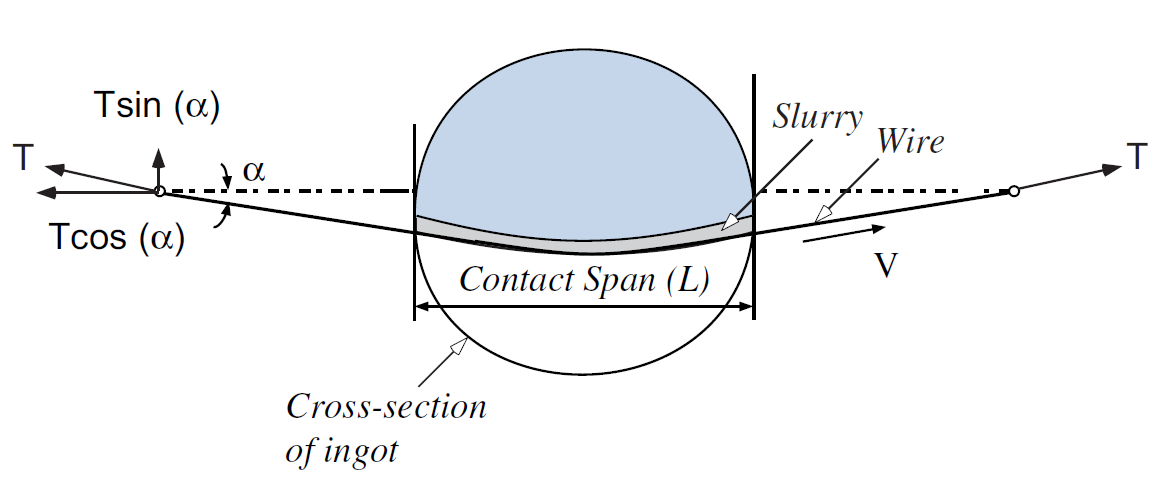
\includegraphics[width=6.0in]{wiresaw-crossection.PNG}
        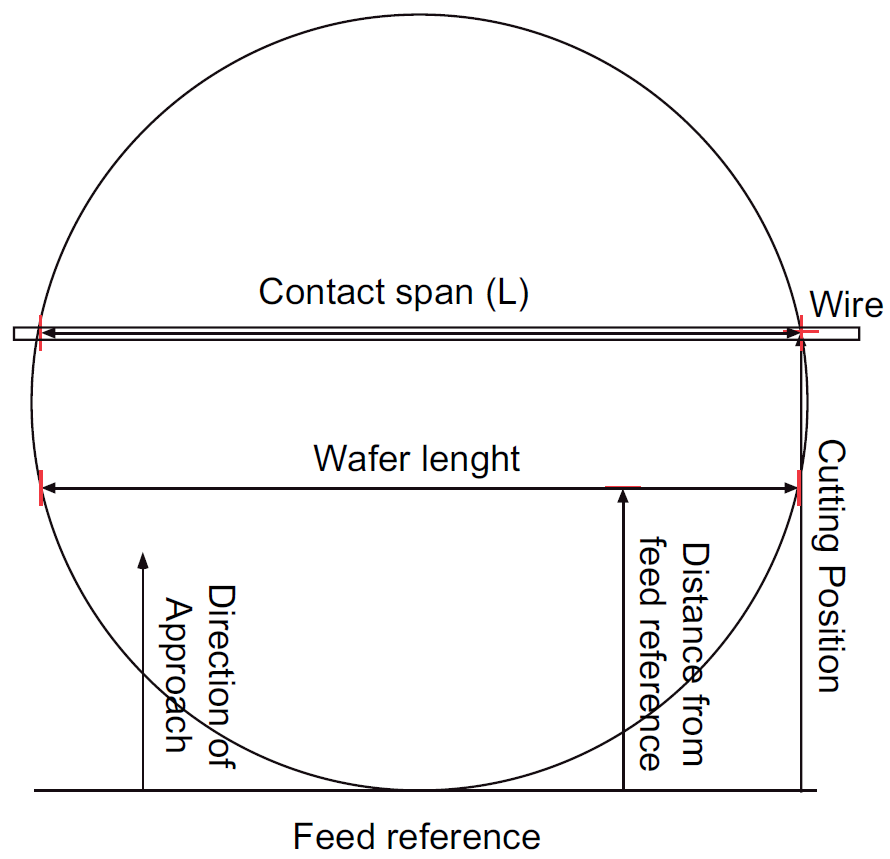
\includegraphics[width=2.5in]{wiresaw-crossection2.PNG}
        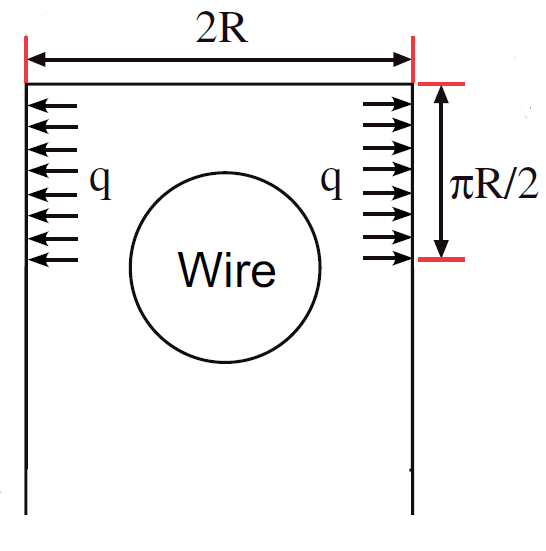
\includegraphics[width=2.5in]{wiresaw-groove.PNG}
        \captionof{figure}{Wire movement}
        \label{fig:wiresawing-crossection}
 \end{minipage}
\subsubsection{Heat Flux}
The most important aspect of thermal modelling of wire-sawing is to the determine the heat flux entering the work piece from the wire and the heat exiting from the new surface formed due to surface convection. Heat flux entering inside the ingot depends upon several factors including wire and slurry parameters. An analytical model has been developed by Bhagwat and Kao [ref] to model this heat flux as a function of power supplied to the wiresaw machine $P$ (\SI{}{W.m^{-2}}), area being machined $A$ (\SI{}{m^{2}}) and a dimensionless quantity $\epsilon$ representing the fraction of power transferred from that is actually being used for slicing.

\begin{equation}
Q = \frac{\epsilon P}{A}
   \label {wire_eq1}
\end{equation}


The power $P$ can be further expressed as 


\begin{equation}
P = Tv
   \label {wire_eq2}
\end{equation}

Where $T$ is the tension set in the wire during slicing, $v$ is the velocity of the wire during sawing. The area being machined can be expressed as

\begin{equation}
A = \pi R L
   \label {wire_eq3}
\end{equation}
Where R is the radius of the groove formed during slicing, L is the contact span. Contact span is the length of wire in contact with the ingot as shown in Figure \ref{fig:wiresawing-crossection}. The dimensionless quantity $\epsilon$ is a function of angle $\alpha$ that it makes with the horizontal axis because of bowing while slicing. The force exerted by the wire can be resolved into horizontal and vertical component. The vertical component of the tension in the is assumed to be responsible for the slicing and can be expressed as $T \sin (\alpha)$. As discussed in Sec. 2.4, the elasto-hydrostatic pressure while wire sawing is a function of contact span length L. Thus, taking these two factors into consideration, the dimensionless constant $\epsilon$ can be defined as 
\begin{equation}
\epsilon = \sin(\alpha) \times L
   \label {wire_eq4}
\end{equation}

$\epsilon$ should also include a constant for the amount of heat dissipating in the slurry. Yamada et al [ref] have estimated that 1/3 to 1/2 of the heat from the wire is taken away by the slurry. However, for this analysis this loss of heat by slurry is ignored for simplicity.  

The flux entering also depends on the length of heat source $l_{s}$ i.e. , as shown in Figure \ref{fig:wiresawing-crossection}, is $\pi R /2 $. During the finite element formulation of this process, however, the flux applied is multiplied with the length of the element $l_{e}$ instead of $l_{s}$. There is an issue in this approach if $l_{e}$ is greater than $l_{s}$ as it supplies extra flux in every step. To balance this, a factor $l_{s}/l_{e}$ is also multiplied to the supplied heat flux. The heat flux increases with cutting depth till the center after which it symmetrically decreases. The increase in flux with the depth of cut till the center is shown in Figure \ref{fig:wiresaw-flux}. 

\noindent
\begin{minipage}[c]{\textwidth}
\centering
        \captionsetup{type=figure}
        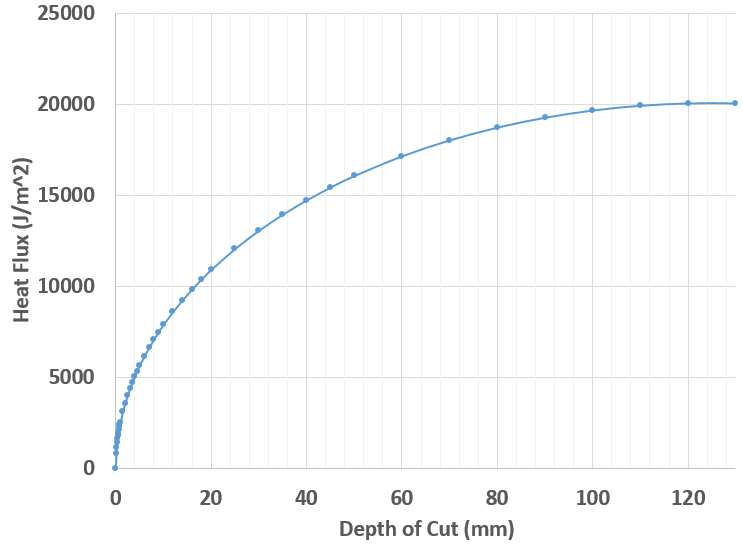
\includegraphics[width=4.0in]{wiresaw-flux.PNG}
        \captionof{figure}{Heat flux with cutting depth}
        \label{fig:wiresaw-flux}
\end{minipage}

\subsubsection{Natural Convection}
During wire sawing simulation, new surface is created at each step of the model. All surfaces that are exposed to the air during slicing, including the newly formed surfaces, are to be applied with natural convection boundary condition. 

Silicon surface has a natural convection coefficient of $h = 5$ \SI{}{W.m^{-2}.K^{-1}} [ref]. But this value can’t be used for the newly formed wafer surfaces. The newly formed wafer surfaces on the work piece is analogous to equally spaced fins, the length which corresponds to the wafer length at a given distance from the feed and height corresponds to the distance from the feed reference. 

The case of natural convection in a Fin has been studied by several researchers [ref-ref]. Harahap and McManus [ref] experimentally found out that convection coefficient decreased rapidly on increase of fin length. Jones and Smith [ref] found out that height of the fin has negligible impact on the convection coefficient of the fin. Chen et al [ref] have analytically solved for convection heat transfer coefficient for a circular annular fin and found it to be a decreasing with decrease in radial distance. For this simulation convection coefficient data is taken from Bhavwat and Kao [ref] which is shown in Figure \ref{fig:wiresaw-h}.  At the cutting position near the feed reference, convection coefficient is 5 \SI{}{W.m^{-2}.K^{-1}} and at the center of ingot it is 0.5 \SI{}{W.m^{-2}.K^{-1}}.

\noindent
\begin{minipage}[c]{\textwidth}
\centering
        \captionsetup{type=figure}
        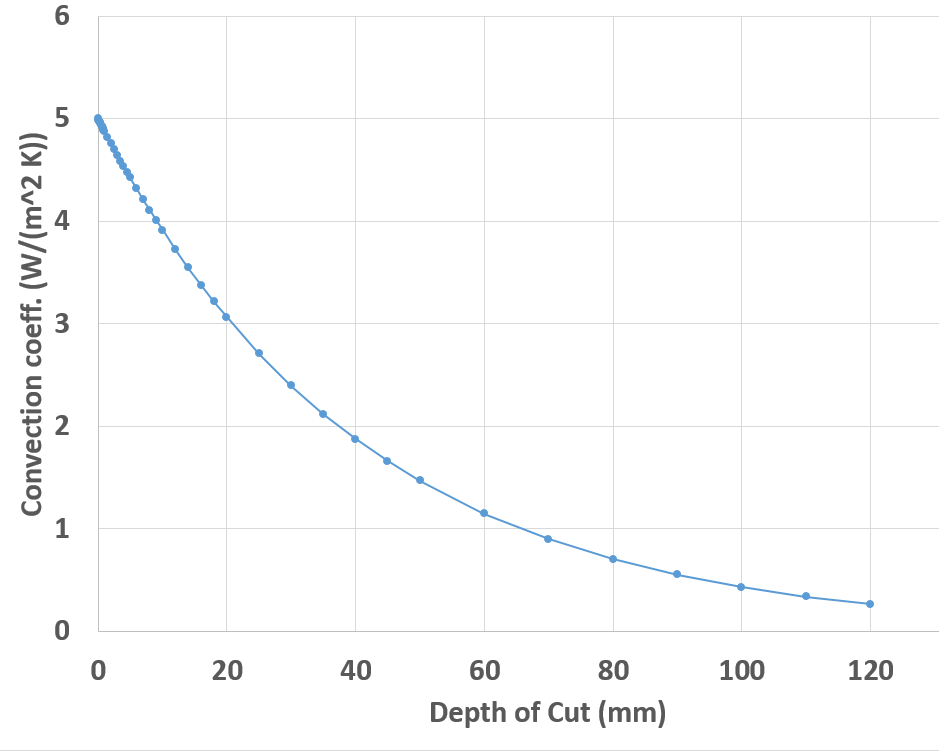
\includegraphics[width=4.0in]{wiresaw-h.PNG}
        \captionof{figure}{Heat flux with cutting depth}
        \label{fig:wiresaw-h}
\end{minipage}

\subsection{Wire Sawing: Displacement Model}

%\subsubsection{Initial Conditions}
Stress, strain and dislocation density results from the casting displacement model are supplied as initial condition for the wire sawing displacement model. Similarly to the casting displacement model, temperature was taken from the wire sawing thermal model at each step using *TEMPERATURE in ABAQUS.  
%\subsubsection{Boundary Conditions}

The mechanical boundary conditions supplied were pinning of nodes at the point where the wire leaves the work piece. This was done because the wafers need to be in fixed contact with some point during the sawing process. 

%Nodes on the surface W1 and W2 where mechanically pinned. This was done because of the way the stress and the strain were mapped from the ingot to the wafer submodel. This will be discussed in more detail while explaining the implementation details of this model in SEC X.X. 

